% =========================================================================
% LaTeX submission template for Advances in Geochemistry and Cosmochemistry
% =========================================================================
% October 2025, the AGC copyediting team

% Do not change the contents of this file!
% This file should only be compiled and will read input from other files.
% All input must be provided in the following files:
% abstract.tex
% authorinfo.tex
% manuscript.tex
% bibfile.bib
% If additional packages are needed for compilation, these must be defined in a file named addpackages.tex
%
% If you encounter compilation errors that you are (reasonably) certain are not due to errors in your own code, there might be a problem with the template which may be specific to your particular LaTeX installation. 
% We recommend using an up-to-date full installation of LaTeX, if possible, and to use pdfTeX as the compilation engine. 
% If the compilation errors persist, please alert the copyediting team at: copyediting@agcj.org
% =========================================================================

% -----------------------------------------------
% General preamble (not to be changed by Authors)
% -----------------------------------------------
\RequirePackage{fix-cm} % solves some encoding problems; must be loaded before \documentclass
\documentclass[12pt, oneside, a4paper]{article}
\usepackage[utf8]{inputenc} % this may be redundant
\usepackage[LGR,T1]{fontenc} % font encoding
\pdfsuppressptexinfo15 % suppress info of imported PDFs
\usepackage{pdfprivacy} % remove sensitive metadata from PDF
\usepackage{setspace} % provides \doublespacing for review

% Base packages and settings
\usepackage{cmbright} % AGC's body typeface
  \renewcommand{\bfdefault}{sb} % use semi bold instead of bold weight
\usepackage{amsmath} % math symbols, may cause definition clashes with some fonts
\usepackage{commath} % provides correctly typeset differential symbols, e.g. \dif 
\usepackage{amssymb} % more math symbols, may cause definition clashes with some fonts
\usepackage{gensymb} % enables \micro command
\usepackage{textcomp} % enables some extra symbols
\usepackage{marvosym} % some more extra symbols, including \Letter and \Email
\usepackage[expansion=false]{microtype} % advanced micro formatting, kerning, hyphenation...
\usepackage[hang, flushmargin]{footmisc} % footnote formatting
  \renewcommand{\thefootnote}{\arabic{footnote}} % use numbers instead of symbols
\usepackage{perpage} % pagewise numbering options
  \MakePerPage{footnote} % from perpage package
\usepackage{graphicx} % graphics
\usepackage{booktabs} % more control over table formatting
\usepackage{siunitx} % SI units
  \sisetup{mode=match,range-units=single, range-phrase=--} % from siunitx package
  \DeclareSIUnit{\amu}{amu} % declaring custom units for use with siunitx package
  \DeclareSIUnit{\annum}{a} % declaring custom units for use with siunitx package
\usepackage{amsmath} % additional math symbols
\usepackage{longtable} % multi-page tables
\usepackage{pgfplots,pgfplotstable} % allows to source table contents from .csv files
\usepackage[version=4]{mhchem} % for chemical formulas outside Math; not compatible with chemsym!
\usepackage{lastpage} % provides LastPage reference
\usepackage[style=iso]{datetime2} % changes date format to ISO 8601
\usepackage[compact]{titlesec} % title formatting
  \titlespacing*{\section}{0pt}{*4}{*1.5} % from titlesec package
  \titlespacing*{\subsection}{0pt}{*2}{*1.0} % from titlesec package
  \titlespacing*{\subsubsection}{0pt}{*2}{*1.0} % from titlesec package
  \titleformat*{\section}{\color{AGC1}\large \bfseries} % from titlesec package
  \titleformat*{\subsection}{\color{AGC1}\bfseries} % from titlesec package
  \titleformat*{\subsubsection}{\color{AGC1}\fontshape{sl} \selectfont} % from titlesec package
\usepackage{xcolor} %custom colors
  \definecolor{AGC1}{HTML}{085766} % defining AGC colors with xcolor package
  \definecolor{AGC2}{HTML}{EDB776} % defining AGC colors with xcolor package
  \definecolor{AGC3}{HTML}{21798A} % defining AGC colors with xcolor package
  \definecolor{AGC4}{HTML}{EAEAEA}   % defining AGC colors with xcolor package
\usepackage{fancyhdr} % provides fancy header options
\usepackage{url} % proper line breaking in urls
  \urlstyle{sf} % set url font to sans serif (default is typewriter)
\usepackage{doi} % solves some problems with doi formatting
\usepackage[elide]{natbib} % the old and stable way of handling bibliographies
  \bibliographystyle{erae} % similar to apalike but with doi (jss2 is more compact but has url and ISSN)
\usepackage{orcidlink} % requires orcidlink version 1.0.4
\usepackage[tmargin=25mm, bmargin=20mm, lmargin=30mm, rmargin=30mm, headsep=10mm, footskip=9mm]{geometry} % set geometry of pages
  \renewcommand{\headrulewidth}{0.5pt} % define width of line under page header
  \renewcommand{\footrulewidth}{0.5pt} % define width of line above page footer
  \renewcommand{\footrule}{\color{black}\hrulefill} % color of footrule
  \renewcommand{\footruleskip}{3mm} % set spacing under footrule
\usepackage{lineno} % provides line numbering
\def\labelitemi{\raisebox{0.35ex}{\tiny$\bullet$}} % defines better default bullet points
\usepackage{enumitem} % format lists
  \setlist{noitemsep, topsep=0pt, leftmargin=*}
\usepackage{newfloat} % define additional floating environments
  \DeclareFloatingEnvironment{fullwidthblock} % use this to place arbitrary content like a float
\renewcommand{\floatpagefraction}{0.85} % sets minimum proportion of floats on page before page becomes float-only; default is 0.6
\IfFileExists{./addpackages.tex}{% -----------------------------------------------
% Space for loading additional packages as needed
% -----------------------------------------------

% ---------------------------------------------------------------------------------
% Set your own hyphenation rules for words that LaTeX hyphenates wrong or awkwardly
% ---------------------------------------------------------------------------------
\hyphenation{geo-chem-istry cosmo-chem-istry} % define custom hyphenation if necessary, can also be use to suppress hyphenation in words
}{} % read extra packages from specified file only if it exists
\usepackage{hyperref} % should be loaded near end of header but before first use, may need to be moved around if it causes problems; to be tested
  \hypersetup{colorlinks=true, linkcolor=AGC1, anchorcolor=black, citecolor=AGC3, filecolor=black, menucolor=black, runcolor=black, urlcolor=AGC1}
  \newcommand*{\colorpageref}[2]{\hypersetup{linkcolor=#2}\pageref{#1}\hypersetup{linkcolor=black}} % necessary for colored text with hyperlinks to override the color override of hyperref
  \renewcommand{\figureautorefname}{Fig.}
  \renewcommand{\tableautorefname}{Tab.}
  \renewcommand{\equationautorefname}{Eq.}


% --------------------------------
% Commands for authorinfo.tex file
% --------------------------------
%\newcommand*{\Titleformat}{\textbf\LARGE}
%\newcommand*{\Titletext}{Manuscript title}
\newcommand*{\Title}[1]{\raggedright\textbf{\LARGE #1}\par \vspace{5mm}} % manuscript title formatting
%\newcommand*{\Title}[1]{\Titleformat #1}
\newcommand*{\Author}[3][]{{\ifthenelse{\equal{#1}{}}{\protect\raisebox{1.25ex}{\large#2\textsuperscript{#3}}} {\protect\raisebox{1.25ex}{\large#2\textsuperscript{#3}\orcidlink{#1}}}}\ \ \setlength\parskip{6pt}} % ORCiD link only appears when given as optional argument
\newcommand*{\CA}{\Letter} % sets the mark for corresponding authors
\newcommand*{\Affil}[2]{{\vspace{-0.3\baselineskip}\small\begin{itemize}\item[\textsuperscript{#1}]{#2}\end{itemize}}\setlength\parskip{0pt}} % authors affiliation formatting
\newcommand*{\Corresp}[2]{{\vspace{0.3\baselineskip}\small \textbf{\Letter\ Correspondence to:} #1:\ \href{mailto:#2}{#2}}} % mail link
\newcommand*{\AltCorresp}[2]{{\small or #1:\ \href{mailto:#2}{#2}}} % mail link
%\newcommand*{\Supp}{None} % default unless changed with \renewcommand*{\Supp}{} in authorinfo.tex
\newcommand*{\Credit}[1]{\vspace{0.3\baselineskip}\small \textbf{Author contributions:} #1} % writing credits
\newcommand*{\Supp}[1]{\vspace{0.3\baselineskip}\small \textbf{Supplementary material:} \url{#1}}


% -------------------
% General page design
% -------------------
\pagestyle{fancy} % sets pagestyle to fancy by default
  \fancyhf{}
  \fancyhead[C]{\selectlanguage{english}\bf\small\color{black} Manuscript submitted to Advances in Geochemistry and Cosmochemistry for review}
  \renewcommand{\headrulewidth}{0.5pt} % defines width of headrule, 0pt removes it altogether
  \renewcommand{\headrule}{\color{black}\hrulefill}
  \fancyfoot[C]{\selectlanguage{english}\bf\small\color{black} page \thepage\ of {\hypersetup{linkcolor=black}\pageref{LastPage}}}
  \renewcommand{\footrulewidth}{0.5pt} % defines width of footrule, 0pt removes it altogether


% ------------------------------------
% Definition of title block appearance
% ------------------------------------
\newcommand{\AGCtitle}{\begin{@twocolumnfalse}\linespread{1.0}\selectfont
  % ----------------------------
% Early career paper indicator
% ----------------------------
% Uncomment the following line if the first author has received their highest degree within the past eight years 
%\noindent \textbf{Early Career Paper}\\[1ex]

% ----------------
% Manuscript title
% ----------------
% Fill in as follows: \Title{The title of the manuscript}
\Title{Statistical chronometry of meteorites revisited}


% ------------
% Author names
% ------------
% Fill in as follows: \Author[ORCiD number]{Full Name}{Affil number}
% The ORCiD number is optional but encouraged
% The Affil number refers to the affiliations given in the next block; should be in order of sequence starting at 1; can be used repeatedly if, e.g., the third author has the same affiliation as the first
% Put each author on a separate line with no blank lines in between
% Mark all corresponding authors with "\CA" after the Affiliation number as in \Author[ORCiD number]{Full Name}{Affil number\CA}
%\Author[]{}{1}
%\Author[]{}{}
\Author[0000-0003-3404-1209]{Pieter Vermeesch}{1\CA}
\Author[0000-0002-1571-0836]{Steven J. Desch}{2}
%\Author{Anonymous}{}


% ---------------------
% Authors' affiliations
% ---------------------
% Fill in as follows: \Affil{Affil number}{Full address}
% The Affil numbers are used in the Author block above
% Comment out for blind review
%\Affil{}{}
\Affil{1}{University College London, UK}
\Affil{2}{Arizona State University, USA}


% --------------
% Correspondence
% --------------
% Fill in as follows: \Corresp{Unique initials of corresponding author}{email address}
% For additional corresponding authors add: \AltCorresp{Unique initials of corresponding author}{email address}
% Multiple additional corresponding authors are possible.
% Please comment out all \Corresp and \AltCorresp lines for initial submission but include them for final submission
\Corresp{PV}{p.vermeesch@ucl.ac.uk}
%\AltCorresp{}{}
%\AltCorresp{}{}


% ---------------
% Writing credits
% ---------------
% List the contributions of all authors according to the Contributor Role Taxonomy (CRediT).
% Use unique initials to identify the authors.
% Choose from the following list of roles: Conceptualization; Data curation; Formal analysis; Funding acquisition; Investigation; Methodology; Project administration; Resources; Software; Supervision; Validation; Visualization; Writing -- original draft; Writing -- review \& editing
% For details see https://credit.niso.org/
% Not all CRediT categories are relevant for every paper, only "Writing -- original draft" is mandatory.
% Comment this info out, if you requested an anonymous review process (blind review).
\Credit{Conceptualization: PV; Data curation: SD; Investigation PV, SD; Methodology: PV, SD; Software: PV; Visualization: PV; Writing -- original draft: PV; Writing -- review \& editing: PV, SD}


% ----------------------
% Data, code, and outputs
% ----------------------
% Uncomment and add web address of data, code, and outputs published at an external repository
%\Supp{} % can be a private review link to a data repository for the purpose of the review process but must be a valid DOI for the final submission
 % comment this in to use the your own authorinfo file
  \vspace{\baselineskip}
  \hrule
  \vspace{\baselineskip}
\end{@twocolumnfalse}\linespread{1}\selectfont}


% ---------------------
% Switches and settings
%----------------------
\usepackage[english]{babel} % adjust this according choice of languages for abstracts
\usepackage[figurename=Figure, tablename=Table, skip=0.25\baselineskip]{caption} %formatting options for captions
\linenumbers % line numbers for proof stage
\usepackage{draftwatermark}
  \SetWatermarkScale{0.6}
  \SetWatermarkColor[gray]{0.96}
  \SetWatermarkText{FOR REVIEW ONLY}
\graphicspath{{./figures/}} %save pictures and graphics in folder 'figures' (must provide valid path)
\clubpenalty10000 % adjusts rigidity or sloppiness of linebreak formatting, 10000=maximum, lower=more sloppy
\widowpenalty10000 % adjusts rigidity or sloppiness of linebreak formatting, 10000=maximum, lower=more sloppy
\displaywidowpenalty10000 % adjusts rigidity or sloppiness of linebreak formatting, 10000=maximum, lower=more sloppy
\tolerance=200 % how much white space is ok at end of line
\hyphenpenalty=5000 % how much we dislike hyphenation


% ---------------------------------------
% End of preamble, beginning of main body
% ---------------------------------------
% ===============================================================
\begin{document} % nothing above this line will appear in the pdf


\AGCtitle % creates the title block

\doublespacing % only affects running text, not text in floats (captions or tables)
\selectlanguage{english}
\subsection*{Abstract}
\newcommand{\tSS}{\mbox{$t_{\rm SS}$}}
\newcommand{\tAl}{\mbox{$t_{\rm Al}$}}
\newcommand{\tMn}{\mbox{$t_{\rm Mn}$}}
\newcommand{\tHf}{\mbox{$t_{\rm Hf}$}}
\newcommand{\tPb}{\mbox{$t_{\rm Pb}$}}
\newcommand{\alratio}{\mbox{${}^{26}{\rm Al}/{}^{27}{\rm Al}$}}
\newcommand{\mnratio}{\mbox{${}^{53}{\rm Mn}/{}^{55}{\rm Mn}$}}
\newcommand{\hfratio}{\mbox{${}^{182}{\rm Hf}/{}^{180}{\rm Hf}$}}


The chronology of the early solar system rests on extinct
(\textsuperscript{26}Al--\textsuperscript{26}Mg,
\textsuperscript{53}Mn--\textsuperscript{53}Cr,
\textsuperscript{182}Hf--\textsuperscript{182}W) and extant
(\textsuperscript{207}Pb--\textsuperscript{206}Pb) chronometers.
These should agree with each other if dating the same events, such as
isotopic closure of these systems in a rapidly cooled achondrite.  If
multiple achondrites formed on different parent bodies, the
chronometers should be concordant across them, assuming isotopically
homogeneous values of ${}^{26}{\rm Al}/{}^{27}{\rm Al}$, ${}^{53}{\rm
  Mn}/{}^{55}{\rm Mn}$ and ${}^{182}{\rm Hf}/{}^{180}{\rm Hf}$.
Testing the homogeneity of these short-lived radionuclides (SLRs) is
often done by comparing a few samples, but really requires a
statistical framework considering many meteorites simultaneously.
Here we discuss two similar statistical approaches.  The first is that
of Desch et al. (2023a,b: doi:10.1016/j.icarus.2023.115607 and
doi:10.1016/j.icarus.2023.115611), which calculates the time of
formation of an achondrite after the start of the solar system ($t=0$,
which happened a time $t_{\rm SS}$ ago), in different isotopic
systems, and takes their weighted mean as the best estimate of the
formation time.  This model was applied to 38 dates across 14
multiply-dated achondrites, adjusting Pb--Pb ages for ${}^{238}{\rm
  U}/{}^{235}{\rm U}$ fractionation during mineral formation.  We
correct an error in their calculation of the goodness-of-fit parameter
and demonstrate that the adjusted formation times show a small but
statistically significant degree of overdispersion with respect to
their analytical uncertainties.  We also introduce a second approach
to statistical chronometry, which is to calculate times of formation
before the present, essentially converting dates into `Pb--Pb times',
using a single offset parameter per isotopic system, estimated by a
weighted regression with a fixed unit slope.  Applying the second
algorithm to the same data compilation yields the same conclusion of
statistically significant overdispersion.  Extending the regression to
a random-effects model allows the excess scatter to be quantified.
The overdispersion of the Pb--Pb ages relative to the extinct
chronometers is greatly reduced after the corrections of Desch et
al. (2023) for uranium isotopic fractionation, from 450--900\,kyr to
50--380\,kyr.  Whether this remaining overdispersion is astrophysical
or analytical in origin is unresolved.  One explanation for this
remaining overdispersion might be variability of SLR abundances.  If
all variations are attributed to this, it would require 0.5 to 7.5\%
(or 40 to 130\%) variations in the ${}^{26}{\rm Al}/{}^{27}{\rm Al}$
ratio, or 2 to 7.5\% (or 5 to 22\%) variations in the ${}^{53}{\rm
  Mn}/{}^{55}{\rm Mn}$ ratio, or 1.4 to 6.8\% (or 3 to 10\%)
variations in the ${}^{182}{\rm Hf}/{}^{180}{\rm Hf}$ ratio (values in
parentheses referring to the uncorrected Pb--Pb ages).  These
relatively small variations are difficult to rule out on purely
astrophysical grounds, but would not explain the persistent
overdispersion even among angrites, which derive from the same parent
body.  This suggests that systematic variations in analysis are at
least partly responsible for the overdispersion of achondrite
formation times.  Routine measurement of ${}^{238}{\rm U}/{}^{235}{\rm
  U}$ in the mineral phases used for Pb--Pb dating, and improvements
in development of isochrons, would test this interpretation.
 % comment this in to use your own abstract file
\section{Introduction} %  % not strictly mandatory but almost universally necessary
\label{sec:intro}

The chronology of the early solar system can be constrained from the
radiogenic decay products of extinct (\textsuperscript{26}Al,
\textsuperscript{53}Mn, \textsuperscript{182}Hf) and extant
(\textsuperscript{235}U, \textsuperscript{238}U) nuclides in
meteorites. The extinct nuclides form the basis of relative
chronometers, which can be used to estimate the age difference between
pairs of meteorites.  In principle, the extant nuclides can be used to
anchor meteorites in absolute time, counting back from the present.
However, in practice the precision of such absolute dates is limited
by the analytical uncertainty of the decay constants
\citep{ludwig2000}. For the
\textsuperscript{207}Pb/\textsuperscript{206}Pb method, this
uncertainty amounts to ca.~9\,Myr ($2\,\sigma$) at 4567\,Ma
(Figure~\ref{fig:lambda_err}).  The decay constant uncertainty is
greatly reduced when calculating the difference between two similar
\textsuperscript{207}Pb/\textsuperscript{206}Pb dates
(Figure~\ref{fig:lambda_err}).  If a different value of the decay
constant is assumed, the ages of both samples are increased or
decreased by a similar amount.  The age {\it difference} is therefore much
more certain than $\pm 9$ Myr.  For example, a 10\,Myr age difference
near the onset of the solar system is associated with a decay constant
uncertainty of only 7\,kyr, as long as all the samples are dated
assuming the same decay constants.  In that case, when comparing
\textsuperscript{207}Pb/\textsuperscript{206}Pb dates within the
4550--4568\,Ma age range, decay constant uncertainties can be safely
ignored, turning the
\textsuperscript{207}Pb/\textsuperscript{206}Pb-method into a relative
chronometer with similar precision as the extinct
chronometers.\medskip

\begin{figure}[!ht]
  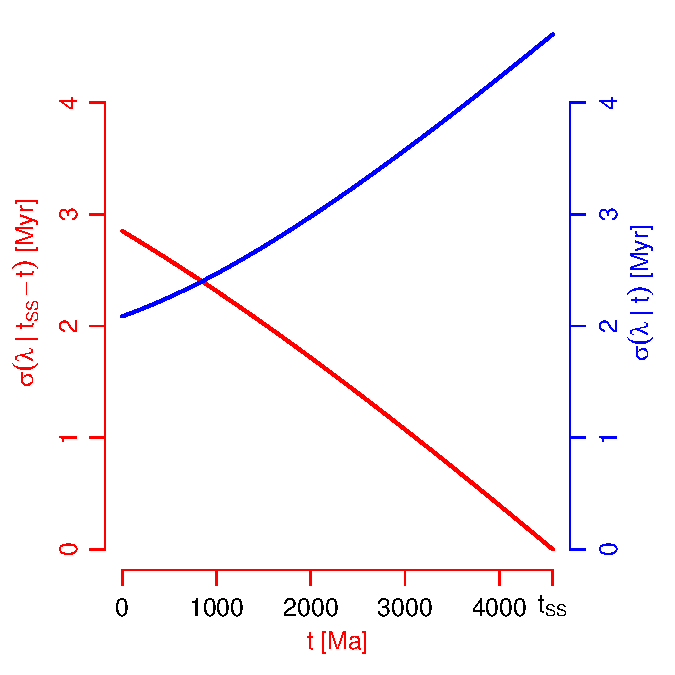
\includegraphics[width=.6\linewidth]{lambda_err.pdf}
  \caption{(blue) uncertainty (standard error) in the inferred
    Pb--Pb age of a sample with true age $t$, due to the uncertainty in
    the decay constants of ${}^{238}{\rm U}$ and especially
    ${}^{235}{\rm U}$; (red) uncertainty in the difference between the
    inferred Pb--Pb age of a sample with true age $t$, and a second
    sample with age $t_{\rm SS}$, Pb--Pb dated using identical decay
    constants which are uncertain.  When used as a relative chronometer
    to date differences in formation times between two objects, the
    uncertainty is small (roughly 1\% of the age difference); but when
    used as an absolute chronometer, the $2\,\sigma$ uncertainty is
    about 9 Myr.}
  \label{fig:lambda_err}
\end{figure}

For a rapidly ($\ll 10^5$ yr) cooled achondrite in which all isotopic
systems reached closure simultaneously, the ages or formation times
derived from each system should agree, assuming the Pb--Pb age of the
solar system, $t_{\rm SS}$, and a particular set of initial values of
${}^{26}{\rm Al}/{}^{27}{\rm Al}$, ${}^{53}{\rm Mn}/{}^{55}{\rm Mn}$,
and ${}^{182}{\rm Hf}/{}^{180}{\rm Hf}$.  The ages or formation times
of a second rapidly cooled achondrite also should agree with each
other.  If the short-lived radionuclides were uniformly distributed in
the solar nebula, the ages of both achondrites would be
self-concordant and concordant with each other, for the same set of
assumed parameters.  The best tests of homogeneity extend this idea to
a basket of achondrites date across multiple systems, comparing
multiple samples simultaneously, using a `statisical chronometry'
approach.\medskip

This paper presents two approaches to this problem.  A first approach
is to establish a chronology for the early solar system counting
forward in time from the start of the solar system, a time $t_{\rm
  SS}$ ago, using the scatter of double-, triple- and quadruple-dated
meteorites around their weighted means (Section~\ref{sec:means}).  A
second approach is to build the statistical chronology counting
backward in time, starting from the present and using linear
regression instead of weighted means
(Section~\ref{sec:regression}).\medskip

In Section~\ref{sec:application}, we apply both approaches to a
dataset of Al--Mg, Mn--Cr, and Hf--W isochrons, and revised Pb--Pb ages, across 14
achondrites, compiled by \citet{desch2023a,desch2023b}. Previous
statistical analysis of this database using the first approach
suggested concordance of the Al--Mg, Mn--Cr, Hf--W and Pb--Pb systems.
After fixing an error in the calculations of
\citet{desch2023a,desch2023b}, we find that in fact the data show a
small but statistically significant amount of excess dispersion.  In
Section~\ref{sec:discussion}, we quantify this overdispersion by
modifying the linear regression method, and discuss the possible
causes of the overdispersion.

\section{Methods} % not strictly mandatory but almost universally necessary
Before discussing the methods, we define the following terms.
\begin{description}
\item{$\tSS$:} the age the solar system, measured backward from the
  present;
\item{$t$:} the time elapsed since the start of the solar system,
  measured forward in time;
\item{$\tAl$, $\tPb$, $\tMn$, $\tHf$:} the Al--Mg, Pb--Pb, Mn--Cr and
  Hf--Cr ages, respectively, measured backwards in time from the
  present;
\item{$\Delta t_{\rm X}$} $= \tSS - t_{\rm X}$, where $t_{\rm X} \in
  \{\tAl, \tPb, \tMn, \tHf\}$;
\item{$\lambda_{26}$, $\lambda_{53}$:} the decay constants of
  \textsuperscript{26}Al and \textsuperscript{53}Mn, respectively;
\item{$\left[{}^{a}\mbox{X}/^{b}\mbox{X}\right]_{\rm SS}$:} the
  ${}^{a}\mbox{X}/^{b}\mbox{X}$ (e.g.,
  ${}^{26}\mbox{Al}/^{27}\mbox{Al}$)-ratio of the solar system at
  $t=0$, a time $\tSS$ ago;
\item{$\left[{}^{a}\mbox{X}/^{b}\mbox{X}\right]_{0}$:} the
  ${}^{a}\mbox{X}/^{b}\mbox{X}$-ratio of a meteorite at the time of
  its formation;
\item{$\sigma[\ast]$:} the analytical uncertainty (estimated standard
  deviation) of $\ast$;
\item{$\chi^2$:} the chi-square statistic for homogeneity;
\item{$\nu$:} the number of degrees of freedom of the chi-square
  distribution under the null hypothesis;
\item{MSWD:} the mean square weighted deviation, defined as MSWD =
  $\chi^2/\nu$.
\end{description}

\subsection{First Approach: $\tSS \rightarrow t$}
\label{sec:means}

\citet{desch2023a} define $\tSS$ as the Pb--Pb age that would be
inferred for a sample that isotopically closed at time $t=0$, defined
to be when the $\alratio$ in the solar system was $(\alratio)_{\rm SS}
\equiv 5.23 \times 10^{-5}$, the value widely accepted as recorded by
CAIs \citep{jacobsen2008}.  Because the Pb--Pb system could be reset
by transient heating events (without resetting the Al--Mg system),
\citet{desch2023a} did not consider this age to be recorded by any
CAI.  Therefore they regarded this as a free parameter that must be
determined, by finding the value of $\tSS$ that minimizes the
differences between $\Delta t_{\rm Al} = \frac{1}{\lambda_{26}} \left(
\ln \left[ \frac{{}^{26}{\rm Al}}{{}^{27}{\rm Al}} \right]_{\rm SS}
-\ln \left[ \frac{{}^{26}{\rm Al}}{{}^{27}{\rm Al}} \right]_{0}
\right)$ and $\Delta t_{\rm Pb} = t_{\rm SS} - t_{\rm Pb}$, for each
achondrite.  To be more specific, given a sample of $A$ achondrites
with both Al--Mg and Pb--Pb dates, \citet{desch2023a} found the value
that minimizes the chi-squared statistic
\begin{equation}
\chi^2 = \sum_{i=1}^{A} \, 
\left( \frac{ \Delta t_{{\rm Al},i} - \Delta t_i }{ \sigma_{{\rm Al},i} } \right)^2 
+\left( \frac{ \Delta t_{{\rm Pb},i} - \Delta t_i}{ \sigma_{{\rm Pb},i} } \right)^2,
\label{eq:chi2}
\end{equation}
where $\Delta t_i$ is the error-weighted mean of $\Delta t_{{\rm
    Al},i}$ and $\Delta_{{\rm Pb},i}$.  By minimizing $\chi^2$, the
optimal value of the free parameter $\tSS$ (which shows up in each
$\Delta t_{{\rm Pb},i}$) is found.\medskip

If the $A$ achondrites are all concordant with each other for the same
value of $\tSS$, and the stated analytical uncertainties are the only
source of dispersion, then $\chi^2$ should follow a chi-square
distribution with $\nu$ degrees of freedom: low values would be
consistent with isotopic homogeneity, but high values $\chi^2 \gg \nu$
would indicate overdispersion of some cause.  The number of degrees of
freedom is $A - 1$.  Essentially, there is one comparison to be made
for each achondrite, and there is one free parameter ($\tSS$).
\citet{desch2023a} incorrectly used $\nu = 2 A - 1$, assuming that the
deviations of $\Delta t_{{\rm Al},i}$ and $\Delta t_{{\rm Pb},i}$ from
$\Delta t_i$ were statistically independent.  In fact, by the
definition of $\Delta t_i$, they are perfectly anti-correlated, and
only one degree of freedom is introduced per achondrite, not two.
Another way to look at it is that there are $2 A$ variables being fit,
with the 1 parameter $\tSS$, but also $A$ free parameters that are the
weighted mean ages $\Delta t_i$, so that $\nu = 2 A - A - 1 = A -
1$.\medskip

Equation~\ref{eq:chi2} can be generalized to more than two
chronometers, as was done by \citet{desch2023b}.  In this case, it is
not necessary that Al--Mg and Pb--Pb dates both exist for every
achondrite; \citet{desch2023b} included in their compilation 14
achondrites that had Pb--Pb ages and data for at least one other
system (Al--Mg, Mn--Cr, or Hf--W).  Here the fit must also
simultaneously optimize $\tSS$, $({}^{53}{\rm Mn}/{}^{55}{\rm
  Mn})_{\rm SS}$, $({}^{182}{\rm Hf}/{}^{180}{\rm Hf})_{\rm SS}$, and
$\lambda_{53}$.  The error-weighted mean $\Delta t_{i}$ is based on
whatever formation times are available for each achondrite.  When
assessing the goodness-of-fit, \citet{desch2023b} assumed $\nu = N-4$,
based on $N$ formation times across the $A$ achondrites, minus the 4
free parameters.  However, the same logic about the weighted means as
an introduced free parameter applies, and the correct number of
degrees of freedom is $\nu = N-A-4$.

\subsection{Second Approach: $t \leftarrow \mbox{present}$}
\label{sec:regression}

It is worth considering whether a different approach might reduce the
number of free parameters, and allow a different assessment of whether
or not the formation times from \citet{desch2023b} are overdispersed.
The first approach defines $\tSS$ as the Pb--Pb age inferred for a
sample that isotopically closed at the time the $\alratio$ ratio in
the solar system (assuming isotopic homogeneity) was a fixed value
$(\alratio)_{\rm SS} = 5.23 \times 10^{-5}$.  As outlined above, this
age is determined using a basket of multiply-dated achondrites to
align the Pb-Pb and Al-Mg chronometers.  Future updates to the basket
would therefore result in new estimates for $\tSS$.\medskip

A mathematically equivalent use of the basket would be to fix $t_{\rm
  SS}$ and treat $({}^{26}\mbox{Al}/{}^{27}\mbox{Al})_{\rm SS}$ as an
unknown.  Alternatively, the two quantities, $t_{\rm SS}$ and
$({}^{26}\mbox{Al}/{}^{27}\mbox{Al})_{\rm SS}$, can be combined into a
single free parameter by expressing the Al/Mg-dates in `Pb/Pb-time',
i.e. by measuring time from the present rather than from $t_{\rm SS}$.
Applying this method to each achondrite $i$:
\begin{equation}
\tAl_{,i} = \tSS - \frac{1}{\lambda_{26}} \, \ln \left( \frac{
  {}^{26}{\rm Al} }{ {}^{27}{\rm Al} } \right)_{\rm SS} +
\frac{1}{\lambda_{26}} \, \ln \left( \frac{ {}^{26}{\rm Al} }{
  {}^{27}{\rm Al} } \right)_{0,i} = {O}_{26} + \frac{1}{\lambda_{26}}
\, \ln \left( \frac{ {}^{26}{\rm Al} }{ {}^{27}{\rm Al} }
\right)_{0,i}.
  \label{eq:A}
\end{equation}
If the two isotopic systems are concordant, then we expect $t_{{\rm
    Al},i} = t_{{\rm Pb},i}$ for each achondrite, and for a plot of
$t_{{\rm Al},i}$ vs. $t_{{\rm Pb},i}$ to be a line of slope 1, with
unknown offset parameter, ${O}_{26}$, which is determined by linear
regression.  The resultant MSWD can be used to determine the goodness
of fit.  The number of degrees of freedom would be $\nu = A-1$, as
before. Any changes to the basket of meteorite dates would change
${O}_{26}$, and hence $t_{{\rm Al},i}$, but $t_{{\rm Pb},i}$ would be unchanged.  This
approach can also be used to compare Pb--Pb ages to Mn--Cr and Hf--W
formation times, just as they are compared to Al--Mg formation times.

\section{Application to the \citet{desch2023b} database}
\label{sec:application}

\citet{desch2023b} compiled $N = 38$ Al--Mg, Mn--Cr, and Hf--W
isochrons and Pb--Pb ages across $A = 14$ achondrites.  In their
detailed survey of the literature, they adjusted Pb--Pb ages as
follows.  First, they recalculated the Pb--Pb dates of some meteorites
by retrospectively adjusting the
${}^{238}\mbox{U}/{}^{235}\mbox{U}$-ratios by 0.125\textperthousand\ to
account for possible U-fractionation between pyroxene and whole rock,
following \citet{tissot2017}.  This adjustment was deemed necessary
because ${}^{238}{\rm U}/{}^{235}{\rm U}$ measurements are almost
always determined from whole-rock samples, whereas the Pb--Pb dating
requires knowledge of the ${}^{238}{\rm U}/{}^{235}{\rm U}$ ratio in
the mineral phase contributing the most radiogenic Pb, generally
pyroxenes.  Second, they recalculated ${}^{207}{\rm Pb}/{}^{206}{\rm
  Pb}$ vs. ${}^{204}{\rm Pb}/{}^{206}{\rm Pb}$ isochrons for a few
achondrites for which certain aliquots were excluded from the
regression without justification.  They showed that equally valid
alternative choices of which aliquots to include led to similar slopes
(and ages), but with much greater uncertainty than had been reported.
After these adjustments, \citet{desch2023a,desch2023b} developed the
database show in Table~\ref{tab:desch}.

\begin{table}[!ht]
\caption{Summary table for the database of
  \citet{desch2023b}. Headers use the following shorthand notation:
  $\mathit{Al}_0 \equiv
  \left(^{26}\mbox{Al}/^{27}\mbox{Al}\right)_0$, $\mathit{Mn}_0
  \equiv \left(^{53}\mbox{Mn}/^{55}\mbox{Mn}\right)_0$,
  $\mathit{Hf}_0 \equiv
  \left(^{182}\mbox{Hf}/^{180}\mbox{Hf}\right)_0$;
  $t_{\rm orig}$ stands for the original Pb--Pb dates extracted
  from the literature; and $t_{\rm adj}$ represents the adjusted
  values used by \citet{desch2023b}.}
\label{tab:desch}
\footnotesize
\begin{tabular}{@{}r@{~}|@{~}c@{~}c@{~}c@{~}c@{~}c@{~}c@{~}|@{~}c@{~}c@{~}c@{~}c@{}}
  sample & $\mathit{Al}_0$ & $2\sigma(\mathit{Al}_0)$ &
  $\mathit{Mn}_0$ & $2\sigma(\mathit{Mn}_0)$ &
  $\mathit{Hf}_0$ & $2\sigma(\mathit{Hf}_0)$ &
  $t_{\rm orig}$ & $2\sigma\left(t_{\rm orig}\right)$ &
  $t_{\rm adj}$ & $2\sigma\left(t_{\rm adj}\right)$ \\ \hline
  D'Orbigny & 3.93 &  0.39 & 3.23 & 0.03 & 7.15 & 0.17 & 4564.42 & 0.12 & 4563.24 & 0.21 \\
  SAH 99555 & 3.64 & 0.18 & 3.28 & 0.17 & 6.87 & 0.15 & 4564.614 & 0.131 & 4563.51 & 0.24 \\
  NWA 1670 & 5.92 & 0.59 & 2.85 & 0.92 & & & 4565.39 & 0.24 & 4564.02 & 0.66 \\
  NWA 1296 & & & & & 7.01 & 0.28 & 4564.2 & 0.45 & 4563.02 & 0.45 \\
  LEW 86010 & & & 1.35 & 0.05 & 4.8 & 0.42 & 4558.55 & 0.15 & & \\
  NWA 4590 & & & 0.85 & 0.4 & 4.63 & 0.17 & 4557.76 & 0.38 & 4557.57 & 0.38 \\
  NWA 4801 & & & 0.96 & 0.04 & 4.52 & 0.16 & 4556.91 & 0.21 & 4556.63 & 0.28 \\
  Angra dos Reis & & & 1.1 & 0.4 & 4.02 & 0.24 & 4556.45 & 0.29 & 4556.26 & 0.29 \\
  NWA 2999 & & & & & 5.43 & 0.34 & 4560.74 & 0.47 & 4560.55 & 0.47 \\
  Asuka 881394 & 13.07 & 0.56 & 3.86 & 0.23 & & & 4564.95 & 0.53 & 4564.76 & 0.53 \\
  Ibitira & & & 1.06 & 0.5 & & & 4556.75 & 0.57 & 4556.56 & 0.57 \\
  NWA 7325 & 3.03 & 0.14 & & & & & 4563.9 & 1.7 & 4563.7 & 1.7 \\
  NWA 2976 & 4.05 & 0.15 & & & & & 4563.16 & 0.57 & 4563.16 & 0.57 \\
  NWA 6704 & 3.15 & 0.38 & 2.59 & 0.34 & & & 4562.76 & 0.26 & 4562.76 & 0.26\\
\end{tabular}
\end{table}

\subsection{First approach}

Applying the first approach to the $A = 7$ achondrites in
Table~\ref{tab:desch}, \citet{desch2023a} found that a value of $\tSS =
4568.42 \pm 0.24$\,Myr minimizes Equation~\ref{eq:chi2}.  They
obtained an MSWD-value of $\chi^2 / \nu = 0.98$ for the optimal fit,
incorrectly using $\nu = 13$.  In fact, $\nu = 6$, so that $\chi^2 /
\nu = 2.12$.  It is worth noting that 95\% of the time, for 6 degrees
of freedom, $0.21 < \chi^2 / \nu < 2.41$, so the 7 achondrites still
can be considered concordant between the Al--Mg and Pb--Pb systems,
even using the correct $\nu$. \citet{desch2023b} then optimized the
fit using the full database, finding the values of $\tSS$,
$({}^{53}{\rm Mn}/{}^{55}{\rm Mn})_{\rm SS}$, $({}^{182}{\rm
  Hf}/{}^{180}{\rm Hf})_{\rm SS}$ and the half-life of ${}^{53}{\rm
  Mn}$ that minimize $\chi^2$.\medskip

Applying an extended version of Equation~\ref{eq:chi2} to the
corrected data of Table~\ref{tab:desch}, \citet{desch2023b} found an
optimal fit, for which they reported a $\chi^2$-value of 47.94 for the
38 meteorite dates. This optimization led to essentially the same
optimal value of $\tSS = 4586.36 \pm 0.20$\,Myr. Assuming $\nu = N-4 =
34$ degrees of freedom, the $p$-value for the chi-squared test is
0.057, which is greater than 0.05 and fails to reject the null
hypothesis that the ages are concordant.  However, as discussed in
Section~\ref{sec:means}, the actual number of degrees of freedom is
$\nu = N-A-4 = 19$.  Using this correct value yields a $p$-value of
0.00043, resulting in a rejection of the null hypothesis.\medskip

Recognizing that the Hf--W date of NWA~4801 was quite divergent, and
also derived from an achondrite with physical indications of
disturbance to the Hf--W system, \citet{desch2023b} present a second
optimization without this point.  Assuming $\nu = 37-4 = 33$, they
reported $\chi^2 = 35.97$, resulting in a $p$-value of 0.33, which
would be consistent with concordancy across the four isotopic systems
and across the 14 achondrites.  However, using the correct $\nu =
N-A-4 = 19$, the $p$-value is 0.011, which contradicts this
conclusion.\medskip

\subsection{Second approach}

We now proceed to subject the data in Table~\ref{tab:desch} to the
second approach.  Figure~\ref{fig:regression_original} compares the
original Pb--Pb dates with the Al--Mg, Mn--Cr and Hf--W dates,
respectively.  For each of the three pairs of measurements, the offset
${O}_{26}$ (or ${O}_{53}$ or ${O}_{183}$) was found by minimizing the
weighted least squares misfit around the 1:1 line, using the algorithm
of \citet{vermeesch2024}.  All three cases exhibit high MSWD-values
and fail the chi-square test for homogeneity.  This indicates that the
data are overdispersed with respect to the analytical
uncertainties.\medskip

There are several potential explanations for the excess dispersion of
the data around the 1:1 lines in Figure~\ref{fig:regression_original}:
(i) heterogeneity of the initial $(\alratio)_{\rm SS}$, $({}^{53}{\rm
  Mn}/{}^{55}{\rm Mn})_{\rm SS}$, or $({}^{182}{\rm Hf}/{}^{180}{\rm
  Hf})_{\rm SS}$ in the regions of the nebula sampled by each parent
body.  \citep[e.g.,][]{bollard2019, krestianinov2023}; (ii) failure of
the different isotopic systems to close simultaneously, due to impacts
or other events on the parent bodies that reset especially the Hf--W
and Pb--Pb systems; or (iii) a variety of analytical discrepancies
leading to incorrect ages based on the data.  The latter could include
improper estimation of the isotopic fractionation of uranium between
different phases, or inappropriate selection of aliquots to build the
${}^{207}{\rm Pb}/{}^{206}{\rm Pb}$ vs. ${}^{204}{\rm Pb}/{}^{206}{\rm
  Pb}$ isochrons, both of which would lead to dispersion in Pb--Pb
ages.  It could also include inappropriate outlier rejection in the
Al--Mg, Mn--Cr or Hf--W isochrons, as well as the Pb--Pb isochrons
\citep{desch2023a,vermeesch2026f}.  Or, it could be due to
inconsistent calibrations made during the collection of data to build
those isochrons.\medskip

\citet{desch2023a,desch2023b} adjusted the Pb--Pb dates in
Table~\ref{tab:desch} in an attempt to correct for analytical errors
(factor iii).  This adjustment does indeed lower the MSWD-value
considerably (Figure~\ref{fig:regression_adjusted}).  Nevertheless,
the three pairwise comparisons still fail the chi-square test.
Therefore the conclusion from the second approach is still that the
data are overdispersed, and for some reason the different chronometers
are not concordant. In Section~\ref{sec:discussion} we extend the
second approach, to treat the various sources of heterogeneity as an
unknown whose effect can be estimated from the data.

\begin{figure}[!ht]
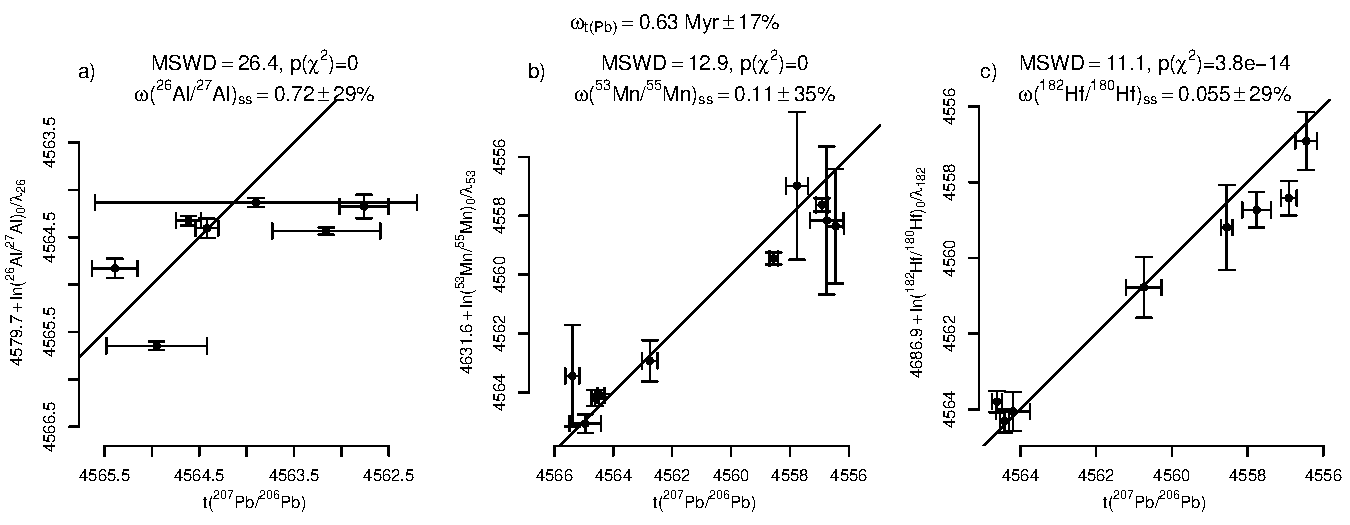
\includegraphics[width=\linewidth]{Desch2_original.pdf}
\caption{Pairwise comparison of the original Pb--Pb dates of
  Table~\ref{tab:desch} with Al--Mg (panel~a), Mn--Cr (panel~b) and
  Hf--W (panel~c) dates for the same, rapidly cooled meteorites. The
  1:1 lines were obtained using the optimal ${O}$-values
  (Equation~\ref{eq:A}). All three datasets are overdispersed around
  this line with respect to the analytical uncertainties
  (MSWD$\,\gg\,1$). $\omega$-values are the estimated standard
  deviations of the excess dispersion, assuming normality
  (Section~\ref{sec:discussion}). This dispersion can either be
  attributed to the Pb--Pb data, or to the initial
  $({}^{26}\mbox{Al}/{}^{27}\mbox{Al})_{\rm SS}$,
  $({}^{53}\mbox{Mn}/{}^{55}\mbox{Mn})_{\rm SS}$ or
  $({}^{182}\mbox{Hf}/{}^{180}\mbox{Hf})_{\rm SS}$-values, or a
  combination. Uncertainties are reported as standard errors.}
\label{fig:regression_original}
\end{figure}

\begin{figure}[!ht]
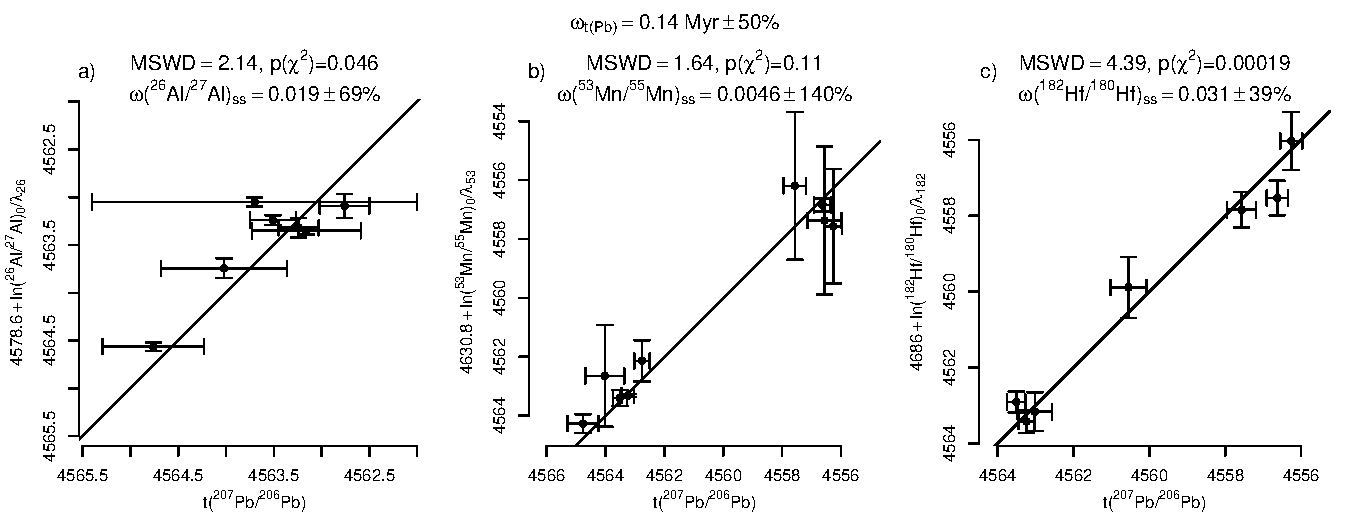
\includegraphics[width=\linewidth]{Desch2_adjusted.pdf}
\caption{Same as Figure~\ref{fig:regression_original},
  but using the adjusted Pb--Pb dates of
  Table~\ref{tab:desch}.\medskip}
\label{fig:regression_adjusted}
\end{figure}

\section{Quantifying dispersion}
\label{sec:discussion}

The observed overdispersion can be mathematically captured by
random-effects models that attribute the excess dispersion to either
the $x$- or the $y$-variables of Figures~\ref{fig:regression_original}
and \ref{fig:regression_adjusted}.  The problem can be formalized by
introducing the following definitions:
\begin{description}
  \item{$t_x(m,i)$:} the `measured' Pb--Pb age of the
    $i$\textsuperscript{th} achondrite;
  \item{$t_y(m,i)$:} the `measured' Al--Mg, Mn--Cr or Hf--W age of the
    $i$\textsuperscript{th} achondrite;
    \item{$\delta_x(i)$:} the random offset between the measured
      $x$-value and the true Pb--Pb age, caused by late isotopic
      closure, or by analytical variations;
    \item{$\delta_y(i)$:} the random offset between the measured
      $y$-value and the true age, due to variations in isotopic
      closure time, or systematic analytical variations, or by
      heterogeneity of $(\alratio)_{\rm SS}$, $(\mnratio)_{\rm SS}$,
      or $(\hfratio)_{\rm SS}$, respectively;
  \item{$x(i) (+ \delta_x(i))$:} the true Pb--Pb age of the
    $i$\textsuperscript{th} achondrite;
  \item{$y(i) (+ \delta_y(i))$:} the true Al--Mg, Mn--Cr or Hf--W age
    of the $i$\textsuperscript{th} achondrite;
  \item{$\epsilon_x(i), \epsilon_y(i)$:} residuals, caused by
    analytical uncertainty.
\end{description}

Using these definitions, we formulate two random-effects models:
\begin{equation}
  \mbox{Model~3x:~}
  \begin{cases}
    t_{x}(m,i) = x(i) + \delta_x(i) + \epsilon_x(i) \\
    t_{y}(m,i) = x(i) + \epsilon_y(i)
  \end{cases}\\
\end{equation}

\noinden and
\begin{equation}
  \mbox{Model~3y:}
  \begin{cases}
    t_{x}(m,i) = y(i) + \epsilon_x(i) \\
    t_{y}(m,i) = y(i) + \delta_y(i) + \epsilon_y(i)
  \end{cases}
  \label{eq:model3xy}
\end{equation}

To keep the problem tractable, it is necessary to make the simplifying
assumption that $\delta_x(i)$, $\delta_y(i)$, $\epsilon_x(i)$ and
$\epsilon_y(i)$ were drawn from normal distributions with zero mean.
For $\epsilon_x(i)$ and $\epsilon_y(i)$, this assumption is
reasonable. For $\delta_x(i)$ and $\delta_y(i)$, that is not
necessarily so. For example, it is possible that there were multiple
reservoirs with distinctly different
$({}^{26}\mbox{Al}/{}^{27}\mbox{Al})_{\rm SS}$-values. However,
Figure~\ref{fig:regression_adjusted}a) only contains 7 double-dates,
which is too small to identify such multi-modality. Therefore, the
simple normal assumption is necessary. The model can easily be
modified to capture more realistic scenarios should a sufficiently
large database of multi-dated meteorites become available in the
future.\medskip

For model~3x, we will assume that the $\delta_x(i)$-values were drawn
from a normal distribution with zero mean and standard deviation
$\omega_{\mathit{t(Pb)}}$ (units: Myr). For model~3y, we will assume
that the $\delta_y(i)$-values were drawn from a normal distribution
with zero mean and standard deviation $\omega_y\lambda_y$ (units:
none), which captures the dispersion of the
$({}^{26}\mbox{Al}/{}^{27}\mbox{Al})_{\rm SS}$,
$({}^{53}\mbox{Mn}/{}^{55}\mbox{Mn})_{\rm SS}$ or
$({}^{182}\mbox{Hf}/{}^{180}\mbox{Hf})_{\rm SS}$-values,
depending on the dataset used to solve the problem. Note that model~3x
can be solved using the combined dataset of Al--Mg, Mn--Cr and Hf--W
measurements.\medskip

If all of the overdispersion is attributed to heterogeneities in the
abundances of short-lived radionuclides, the level of overdisperion is
explained by:
\begin{enumerate}
\item 0.5--7.5\% heterogeneity of the
  $({}^{26}\mbox{Al}/{}^{27}\mbox{Al})_{\rm SS}$-ratio (at $2\sigma$,
  i.e. $\exp[\ln(0.019)\pm{2\times0.69}]$;
  Figure~\ref{fig:regression_adjusted}a).
\item 0.0--7.6\% heterogeneity of the 
  $({}^{53}\mbox{Mn}/{}^{55}\mbox{Mn})_{\rm SS}$-ratio;
\item 1.4--6.8\% heterogeneity of the
  $({}^{182}\mbox{Hf}/{}^{180}\mbox{Hf})_{\rm SS}$-ratio.
\end{enumerate}
If one attributed the overdispersions in the Al--Mg, Mn--Cr, or Hf--W
systems to analytical variations such as differences between groups in
calibrations, then the same variations would apply. If the
overdispersion is attributed to variations in the time of isotopic
closure, of the Pb--Pb system in particular, then the data are
explained by:
\begin{enumerate}
  \setcounter{enumi}{3}
\item 50--380\,ka excess dispersion in the Pb--Pb data.
\end{enumerate}
The same excess dispersion in the Pb--Pb data would apply if the
variations were attributed to analytical problems, such as improper
correction for uranium isotopic fractionation, or over-zealous outlier
rejection, which unduly promotes precision over accuracy
\citep{vermeesch2026f}.  We note that if the original Pb--Pb data are
used, then the dispersion increases to 40--130\% for
$({}^{26}\mbox{Al}/{}^{27}\mbox{Al})_{\rm SS}$, 5--22\% for
$({}^{53}\mbox{Mn}/{}^{55}\mbox{Mn})_{\rm SS}$, 3--10\% for
$({}^{182}\mbox{Hf}/{}^{180}\mbox{Hf})_{\rm SS}$ and 450--900\,kyr for
$t_{\rm Pb}$. We also note that all the Hf--W data in
Table~\ref{tab:desch} were obtained from angrites, which are thought
to derive from a common parent body. Their overdispersion therefore
cannot be attributed to nebular heterogeneity, suggesting instead that
it reflects analytical effects. These effects could apply to the Hf--W
data, the Pb--Pb data, or both.

\section{Conclusion}
\label{sec:conclusion}

In this paper we have presented two equivalent approaches to
statistical chronometry, using an existing compilation of multi-dated
meteorites originally presented by \citet{desch2023b}.  The first
approach tracks events forward in time from $\tSS$, which is treated
as an unknown parameter, and is defined to be when $(\alratio)_{\rm
  SS} = 5.23\times{10}^{-5}$.  Optimal values were found for
$(\mnratio)_{\rm SS}$ and $(\hfratio)_{\rm SS}$ at $t=0$; the Pb--Pb
age of $t=0$, $\tSS$; and the decay constant $\lambda_{53}$.  The
optimal values found by \citet{desch2023b} are unaffected by the
number of degrees of freedom, but the goodness of the fit is.  After
using the correct number of degrees of freedom, this approach reveals
a small but statistically significant dispersion between the extinct
and extant chronometers, even after adjustment for
\textsuperscript{238}U/\textsuperscript{235}U fractionation.\medskip

The second approach uses bivariate linear regression of doubly-dated
meteorites to assess the concordance of the meteorite database. It
does not treat $\tSS$, $(\mnratio)_{\rm SS}$, and $(\hfratio)_{\rm
  SS}$ as explict unknowns, but instead converts the
$\ln\left(^{26}\mbox{Al}/^{27}\mbox{Al}\right)_0$,
$\ln\left(^{53}\mbox{Mn}/^{55}\mbox{Mn}\right)_0$ and
$\ln\left(^{182}\mbox{Hf}/^{180}\mbox{Hf}\right)_0$ logratios to
absolute ages in `Pb--Pb time' using a linear transformation
(Equation~\ref{eq:A}).  Applying the second approach to the database of 
\citet{desch2023a, desch2023b} leads to the same conclusion
as the first approach, that there statistically significant dispersion
of the extinct and the extant chronometers. Adjustment of the Pb--Pb
dates for \textsuperscript{238}U/\textsuperscript{235}U fractionation
reduces the overdispersion but does not completely remove it.\medskip

The regression approach marks a step forward in the development of a
statistical chronometry for meteorites, by going from a simple test
for statistical homogeneity, to the quantification of heterogeneity.
This is important because, to paraphrase statistician George Box ``all
effects are significant (in some decimal place)''.  Given a
sufficiently large or sufficiently precise database of multi-dated
meteorites, even the smallest degree of heterogeneity eventually
becomes detectable. The chi-square test cannot by itself determine the
cause of the overdispersion, but is a useful tool.  The overdispersion
could be physical: the radionuclides could be heterogeneously
distributed among achondrite parent bodies, or the isotopic systems
may have closed at different times or been disturbed.  Or the
overdispersion could be analytical, due to discrepancies between
groups in how isochrons are built.\medskip

Physical causes can be tested by examining the angrites separately,
because they formed from the same parent body. Assuming that these
meteorites remained undisturbed after their formation, their extinct
and extant chronometers should be concordant. However, eight paired
angrite Hf--W and Pb--Pb dates show that this is not the case.  This
suggests the presence of analytical bias in the isotopic ratio data.
Further investigation of these conclusions would benefit from improved
analytical and statistical techniques.  Analytical improvements
include the addition of \textsuperscript{238}U/\textsuperscript{235}U
measurements in the same mineral phase as the Pb-isotope
measurements. Although this is challenging to do in small or U-poor
samples, it is highly beneficial as it removes the need for the
nominal 0.125\textperthousand\ correction applied by
\citet{desch2023a,desch2023b} to many of the meteorites in
Table~\ref{tab:desch}.  Statistical improvements include a more
rigorous selection of aliquots to include in Pb--Pb isochrons.  For
example, \citet{desch2023a} present a detailed discussion of
\citet{schiller2015}'s Pb--Pb dataset for NWA~1670 and show that there
are at least three statistically equivalent ways to form an isochron
through these data, with significantly different ages. To solve this
problem, it would be useful to abandon the binary notion that aliquots
fall either `on' or `off' the concordia line. A statistically more
rigorous approach would be to assign a finite probability to both
categories for each aliquot, similar to the random effects model of
Section~\ref{sec:discussion}.\medskip

The future addition of more multi-dated meteorites to compilation of 
\citet{desch2023b} will make it possible to replace the
simple random effects model of Section~\ref{sec:discussion} with more
realistic alternatives. For example, given a sufficient number of
multi-dated NC and CC chondrites, it would be possible to quantify the
within-group and between-group variability of these two meteorite
classes.  Thus, the nascent field of statistical chronometry has the
potential to test physics-based predictions of solar-system formation
and provide new insights into its temporal evolution.

\section{Acknowledgements} % mandatory

We thank the reviewers for feedback.

\section{Data, code, and outputs availability}

\url{https://github.com/pvermees/supplements} contains all the data
and code used to reproduce this manuscript.

\section{Competing interest}

The authors declare no conflicts of interest regarding this
publication.
 % comment this in to use your own manuscript file

{\footnotesize
  \bibliography{bibfile.bib} % comment this out to use your own abstract file
}

\end{document} % nothing below this line will appear in the pdf
% =============================================================
